\label{sec:face_fiducial_detection}
In this section, we first outline our formulation in section~\ref{subsec:formulation}, followed 
by our algorithm for fiducial detection.
Briefly, given an input image, candidate algorithms return vectors of locations of
various fiducials for that image. Given the output of each of the candidate algorithms, our task
is to identify a set of fiducials that best represent the face in the input image. This can be done
by either selecting the \emph{entire} output of \emph{one} of the candidate algorithms, or by
selecting \emph{individual} fiducials from the various outputs of candidate algorithms to form a facial
structure of our own. In order to do this, we first identify a set of \emph{exemplars} from the
training dataset, that serve as guidelines on how a face should look like, both in shape and
appearance. Our approach is to then \emph{match} candidate algorithm outputs to exemplars from the
training dataset, in order to \emph{select} the best output for the given image.
Our algorithm has two main components: \emph{exemplar selection} (section~\ref{subsec:exemplar_selection}) and
\emph{output selection} (section~\ref{subsec:output_selection}, section~\ref{subsec:optimization}). A flowchart of our approach
is illustrated in Figure~\ref{fig:outline}.

\begin{figure*}
  \centering
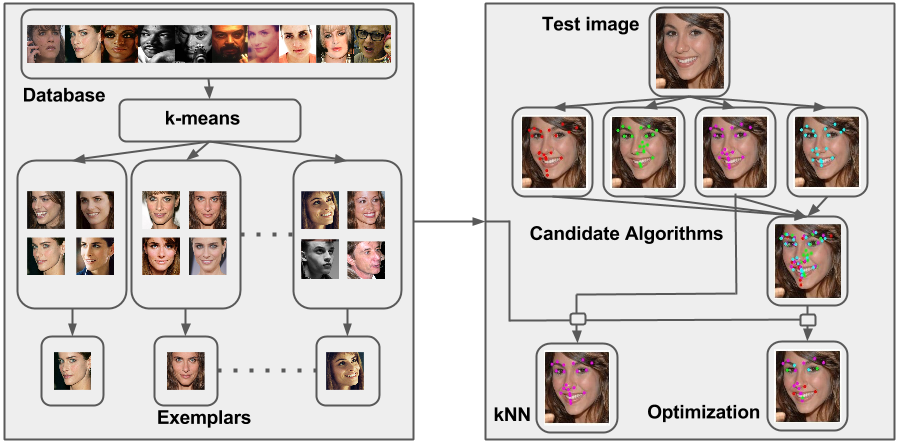
\includegraphics[width=6.0in, height=2.8in]{fid/figures/method.png}
\caption{Left box pictorially represents exemplars selection. Right box represents our two algorithms for output selection. One by using kNN approach and other using optimization. Best viewed in color.}
\label{fig:outline}
\end{figure*}

